\documentclass[11pt]{article}
\usepackage[pdftex]{graphicx}
\usepackage[utf8]{inputenc}
\usepackage{lmodern}
\usepackage{listings}
\usepackage[T1]{fontenc}
\usepackage{caption}
\usepackage{xcolor}
\usepackage{tabularx}


\DeclareCaptionFont{white}{\color{white}}
\DeclareCaptionFormat{listing}{%
	\parbox{\textwidth}{\colorbox{gray}{\parbox{\textwidth}{#1#2#3}}\vskip-4pt}}
\captionsetup[lstlisting]{format=listing,labelfont=white,textfont=white}
\lstset{frame=lrb,xleftmargin=\fboxsep,xrightmargin=-\fboxsep}




% Set the default font
\renewcommand*{\familydefault}{\sfdefault}

% Enable Hyperlinking of TOC entries
\usepackage{hyperref}
\hypersetup{
    linktoc=all
}


% Set margins
\setlength{\textheight}{8in}
\setlength{\oddsidemargin}{.125in}
\setlength{\textwidth}{6.25in}

% Set up BrainGrid Logo as Background Picture (for use in the Title Page)
\usepackage{eso-pic}
\newcommand\BackgroundPic{%
\put(0,0){%
\parbox[b][\paperheight]{\paperwidth}{%
\vfill
\centering

\includegraphics[width=\textwidth,height=4.00in,% % Come up with a better way to restrict the height of the image so that it is below the 
keepaspectratio]{./logos/logo.png}%
\vfill
}}}

\mdseries 
\begin{document}
\AddToShipoutPicture*{\BackgroundPic}
\title{BrainGrid\\Documentation}
\author{Kawasaki, Fumitaka \and Stiber, Michael}
\date{} %Doesn't show the date

\maketitle

\pagebreak

%------------------------------------- Abstract Section
\begin{abstract} \mdseries 
BrainGrid is an open-source neural-network simulator that is intended to aid scientists and researchers by providing prebuilt code that can be easily modified to fit different models. The program also offers the ability to easily transition to a GPU-centered with little additional work, and providing a potential speedup of up to a twentieth of the original runtime.

\begin{center}
	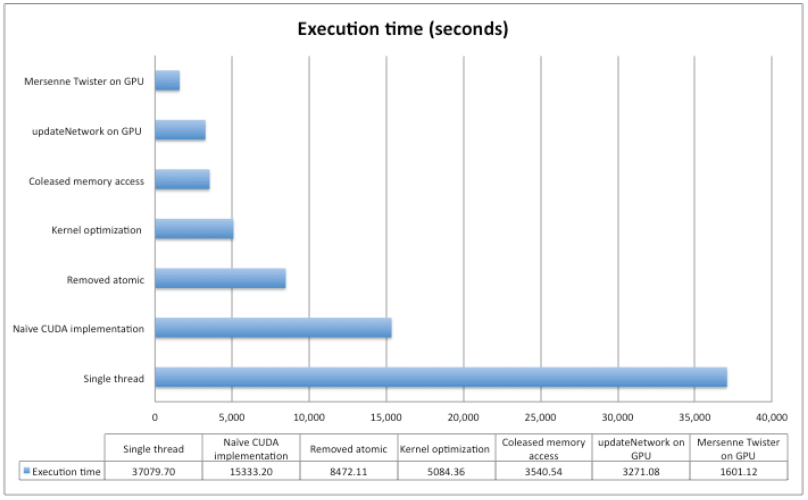
\includegraphics[width=\textwidth]{./images/SpeedComparison.PNG}
\end{center}

\noindent \mdseries The project began as an attempt to reduce the runtime of a simulation of a Leaky Integrate-and-Fire with more than a thousand neurons from two-thousand hours to a much more manageable runtime. Therefore, the program by default comes with a Leaky Integrate-and-Fire simulation preprogrammed. 
\end{abstract}
\pagebreak


%------------------------------------- Table of Contents
\tableofcontents
\pagebreak

%------------------------------------- Linux Crash Course
\section{Linux Crash Course} \mdseries 

% This document assumes a tab-width of 4 characters!!! Formatting will be skewed otherwise!

\subsection{Introduction} \mdseries 
Chances are, many readers will already be familiar with how to use linux or another unix like system.  If this is the case than you are welcome to skip this entire section. However, more than likely there will be at least a few who aren't.  This section is for them, and if it helps at least one person get started faster, then it has served its purpose.

This section is not designed to be the absolute authority on Linux, but is instead designed to introduce the reader to what they may need to begin working on this project in as efficient a way as possible.  There will be an overview of the terminal, directory and file system, useful commands (programs), and hopefully any "gotcha's" that may crop up.  Basically, I wanted to be longer than a blog, but shorter than a book.
	

\subsection{Terminal}
\subsubsection{Quick Introduction} \mdseries
Strictly speaking, you will likely be using a terminal emulator such as Bash (Bourne-again shell), but I'll try to leave semantics aside.  The terminal (aka: command line, bash prompt, shell, TTY) is where the magic happens in Linux (as well as any other *nix OS).  Here, you can run programs, modify files, view the contents of directories, run scripts, and even play games.  When you first open up a terminal you will be presented with a prompt followed by a cursor, though not very interesting or inviting I'm afraid.  Generally the prompt will have the following form: \\
	
\begin{lstlisting}
$ username@hostname:currentdirectory$
\end{lstlisting}
	
A specific example may be the following: \\

\begin{lstlisting}
$ foo@bar:~$
\end{lstlisting}
	
In the above prompt, foo is your username, bar is the hostname or computer name, the tilde '\textasciitilde'  is a shortcut representing your home directory, and the dollar-sign '\$' is just to indicate that you are running as a non-root user.  You are actually quite able to edit the prompt to your liking, and I highly recommend that you do.  My recommendation is not because it's cool, or to show off, but because there is a very practical reason; color.  The standard prompts are generally grey on grey on grey on...  The prompt is grey, the output from commands and programs is grey; you get the picture.  When working in a purely text environment it can be very easy to lose your place.  Actually your place is at the very end of the text block where you see a blinking cursor, but there will invariably be some point where you care about the output above (e.g. when you print out the contents of a directory).

The prompt is defined by the environment variable 'PS1' (without quotes).  You can edit this by appending it to the end of your ~/.bashrc file (remember the tilda is your home directory).  The dot '.' in the previous file makes the file hidden.  The PS1 prompt which I use was an idea shamelessly stolen from someone who shamelessly stole the idea from someone else.  I will provide it here for you to shamelessly steal ;-).  Just copy the following line in its entirety to the end of your ~/.bashrc file.

% Need to figure out a way to allow the unicode characters in the below string....
%	\begin{lstlisting}
%	PS1='\[\e[0;33m\]┌─[\[\e[0;36m\]\u@\h \@\[\e[0;33m\]]──[\[\e[0;36m\]\w\[\e[0;33m\]]\n└─■ \[\e[0m\]'
%	\end{lstlisting}
	
It's a multi-line prompt that is colored so you can easily see where the last command was.  The multiple lines are simply to allow a more complete path to be displayed.


\subsubsection{Running Commands}
\mdseries \noindent Running commands is simple in Linux, all you have to do is call the command from the command line.  For example, if I wanted to list the contents of the current directory, I would run the following command:

\begin{lstlisting}
$ ls
\end{lstlisting}

\mdseries \noindent If I wanted to run Firefox, I would run the following command:
	
\begin{lstlisting}
$ firefox
\end{lstlisting}
	
\mdseries \noindent Yes, it's that easy!  Now for running BrainGrid you would do something like the following:

\begin{lstlisting}
$ ./growth -t config/test-medium-2.xml
\end{lstlisting}
	
\mdseries \noindent Breaking it down, you need to specify the complete path when executing a program that is not in your systems PATH.  While it doesn't appear that we have specified the entire path to the file we actually have.  The dot character '.' above is a *nix shortcut to the present working directory.  The '-t' is a flag and is read in as a parameter.  If you haven't done much command line work in the past, you may have wondered what the 'argc, and argv' arguments were in your main() function.  In short, these are the command line parameters that you pass when executing your program.  The '-t' parameter itself requires another parameter, the configuration file which, we have specified in our command above.  Note, that the configuration file can be a relative path, whereas your program had to be an absolute path.


\subsubsection{Environment Variables} \mdseries 
\mdseries \noindent The terminal utilizes a number of different environment variables to hold certain configurations.  The most important to us are listed below:
\begin{lstlisting}
$HOME
$PS1
$PATH
$LD_LIBRARY_PATH
\end{lstlisting}
	
\mdseries \noindent They are pretty self-explanatory, so I won't go into detail about what each is.  If you wish to view what is stored in each of these variables just run the following command:

\begin{lstlisting}
echo \$VARIABLE
\end{lstlisting}
	
\mdseries \noindent where 'VARIABLE' is the particular environment variable you wish to see.  For example:

\begin{lstlisting}
$ echo \$PATH
\end{lstlisting}


\subsubsection{Pipes and Redirects and the Universal Interface} \mdseries 
\mdseries \noindent In Linux the universal interface is text; it is passed around and modified in any imaginable way!  Let's say you wanted to pass the output of program "a" into program "b".  You would do so with the vertical bar character '|' as follows:
	
\begin{lstlisting}
$ ls | grep "foo"
\end{lstlisting}
	
\mdseries \noindent What the above is doing is sending the standard output of the "ls" command to the standard input of the "grep" command.  The grep command is then searching the input for the substring "foo."  You can chain any number of programs together in this way.  Remember "cin" and "cout" in C++? These are the exact samething.

\mdseries \noindent To dump the output of a program to a file you would use the redirect command such as the following:

\begin{lstlisting}
$ ls > directory-list.txt
\end{lstlisting}
	
\mdseries \noindent This will send the list of the files and folders in the current working directory to a file called "directory-list.txt".  Now, this will send anything indiscriminantly, but let's say you wanted to get a bit more specific.  Say you wrote a program that printed some messages to standard error and others to standard out.  You could independently redirect each of these to a separate file.  "2>" will redirect standard error, and "1>" will redirect standard out.

\begin{lstlisting}
$ ./foo 1> foo.out 2> foo.err
\end{lstlisting}
	
The above, will send the standard output to a file called "foo.out" and the standard error to a file called "foo.err".  Simple enough :-).

	
\subsection{Directories and the Filesystem} \mdseries 
\subsubsection{Main Overview of the Filesystem} \mdseries 
The filesystem of Linux is quite different from that of Windows.  Linux does not have a 'C' drive or 'D' drive, instead everything is a file (yes, even directories are a type of file).  The root of any Linux filesystem is simply '/'.  Yup, that's it, no fancy "C:\" here!  Another important note is that files don't get installed to their own directory, and there is a good reason for this.  In the golden days of Unix, disk space was especially limited so programs shared all libraries.  Two programs need the ncurses library? That's fine, we only need one copy of ncurses.  This means that disk space is saved by eliminating duplicate pieces of software.  The obvious downside is that all software must use the same library(ies).  Also, it is difficult to have multiple versions of the same file on your computer.  We will see this later when we go over installing CUDA.  Now, what are the important libraries?  The ones you will most likely be concerned with are as follows:

\begin{tabularx}{\textwidth}{ | c | X | }
	\hline
	\textbf{Directory}	& \textbf{Description} \\
	\hline
	/usr		& The "user" directory \\
	/usr/lib	& The most common library directory (though there are several others) \\
	/usr/bin	& The most common binary directory.  This is where most executables are actually stored \\
	/usr/local	& The /usr/local directory is where custom software *should* be installed.  This is rarely used anymore as it is trivial to make packages which a package manager can install.  As we will see later, CUDA, in keeping with tradition, installs here. \\
	/home		& This is where the users home directories are located \\
	/var		& This is the "variable" directory.  Any log files will generally be located here (/var/log). \\
	/dev		& This is the "device" directory.  Your disk may likely be mounted to /dev/sda1 and your optical drive will likely be mounted to /dev/sr0. \\
	\hline
\end{tabularx}

\subsubsection{Directory Delimiter} \mdseries
A few notes on directories.  First notice that all directory separations are the forward slash '/'.  This is due to the backslash '\' character being reserved for escaping characters.  

\subsubsection{Directory and File Naming (Case, Spaces, and Style)} \mdseries
Note a that the directory names in the previous list are all lower case.  This raises two points: first, directories are case sensitive; second, *nix gurus hate to press the Shift key.  No really, they're lower-case to make typing easier.  It's a style I definitely recommend adhering to.  Finally, try to avoid spaces in file names.  This is not verboten, but avoiding spaces will, in general, make your life easier.  You see, if you create a directory called "foo bar" and then try to change directory into it with the following command:

\begin{lstlisting}
$ cd foo bar
\end{lstlisting}

It will fail miserably.  This assumes of course that the directory "foo bar" already exists; creating it in that above fashion would also fail.  Now to get around this you either need to put the entire directory path in quotes, or escape the space with the backslash character.  See the following for examples of each.

\begin{lstlisting}
$ mkdir "foo bar"
$ cd foo\ bar
\end{lstlisting}

I recommend using the minus character '-' as separator between multi-word names.  The obvious alternative is the underscore character '\_' (hehe, looks like a face :P), but we here at BrainGrid would like to avoid carpal-tunnel syndrome.  I mean let's face it, does anybody actually like pressing the Shift key?  It's either an awkward pinkey stretch, or a hand movement the could otherwise be avoided by just sticking with a simple '-' character.  


\subsubsection{Directory Shortcuts} \mdseries
Here are a few directory shortcuts.  You have already seen essentially how they are used, and you will see more examples later.

	.	Current directory (current working directory)
	..	Parent directory
	~	Your home directory


\subsubsection{Line Endings} \mdseries
Tne endings in Linux are a bit different than those on Windows.  Linux uses '\textbackslash n' the newline character to end a line.  Windows uses '\textbackslash r\textbackslash n' the carriage return followed by a new line to end a line in a file.  While most text editors are smart enough to know the difference and automatically adjust, there are some that don't.  As a result a file created on Windows when opened on Linux may appear to have extra blank lines added in.  Conversely, a file created on Linux and then opened on Windows may appear to have now new lines at all, making the full text of the document on a single line.


\subsection{Useful Commands (Programs)} \mdseries
If you've been introduced to Linux before you've probably been told to "run command x" or "run command y."  These "commands" are really just tiny programs... Actually, many of them are quite large and complex such as gcc.  Anyways, without further adoo, I present to you a list of the most useful (according to me) Linux commands!  Note each one will have a more detailed description and examples so that you will be sure to not be lost.

\begin{tabularx}{\textwidth}{ | c | X | }
	\hline
	\textbf{Command}	& \textbf{Description} \\
	\hline
	cd		& change directory \\
	ls		& list contents of directory \\
	pwd		& print working directory \\
	mv		& move [a] to [b] (this is also how you rename things) \\
	cp		& copy \\
	rm		& remove \\
	mkdir	& make directory \\
	rmdir	& remove directory \\
	touch	& alter the time stamp of a file, also used to create a file \\
	man		& manual (view the included documentation for programs) \\
	make	& runs a Makefile which will (among other things) compile your code \\
	ssh		& login remotely to a linux machine using a secure shell (ssh) \\
	sftp	& Transfer a file securely from a remote *nix machine (secure ftp) \\
	screen	& Allows you to detach a currently running process so that it may run to completion in the background. \\
	exit	& Self explanatory.  It will exit your session.  If you're logged in it will log you out, etc. \\
	find	& Searches the provided path for the given file or directory \\
	which	& Returns the path of an executable for the given command.  \\
	echo	& Will echo a string to the command line (more useful than you might imagine). \\
	chmod	& Changes the mode of a file (for example, to make a file executable) \\
	chown	& Changes the ownership of a file \\
	tar		& Archiver for files \\
	\hline
\end{tabularx}
		
Just a quick reminder on the way commands are presented.  The command is always prefaced by "\$ ".  This is just to show that you are executing the command as a regular user, nothing more.

\subsubsection{cd} \mdseries
This is the change directory command, and will change into either a relative or absolute directory.  An absolute directory will always begin with the forward slash '/', and a relative directory will never begin with the forward slash character.  This will hold true for all programs.

\begin{lstlisting}
$ cd ../
$ cd ~ 
$ cd ~/foo-bar	#
$ cd ../bar
\end{lstlisting}
	
The above commands do the following:
	\begin{itemize}
		\item Change into the parent directory
		\item Change directory into your home directory
		\item Change into a directory called "foo-bar" located in your home directory
		\item Change into a sibling directory called "bar"
	\end{itemize}

\subsubsection{ls} \mdseries
This is the list command.  It will list the contents of the current working directory.  There are different parameters (flags) you can pass to it to show greater or lesser detail.
	
\begin{lstlisting}
$ ls
$ ls -l
$ ls -a
$ ls -al
\end{lstlisting}
	
The above commands do the following:
	\begin{itemize}
		\item List the current directory
		\item List the current directory with additional information about each file / folder
		\item List the current directory including hidden files and folders
		\item Combines the above two commands to provide a detailed list of all files and folders in the current working directory
	\end{itemize}

\subsubsection{pwd} \mdseries
This is the "Print Working Directory" command.  You were wondering why I kept using the phrase "current working directory" weren't ya? ;-).  It does just that, and is generally fairly useless...  The reason for this is that most command prompts will show you your current directory, at least in part.  The PS1 provided above will display the entire path.  However, in the event that your prompt does truncate the path you can get your current working directory by just executing the above command.  You may also like to use this command in conjunction with the echo command to dump the output to a file for use elsewhere.

\begin{lstlisting}
$ pwd
\end{lstlisting}

The above commands do the following:
	\begin{itemize}
		\item Print the working directory
	\end{itemize}
	

\subsubsection{mv} \mdseries
This is the move command.  It will move a file or directory from "a" to "b".  Additionally this is how you rename files or folders on the command line.

\begin{lstlisting}
$ mkdir foo
$ touch foo/bar.txt
$ mv foo bar
$ mkdir foo 
$ mv bar/bar.txt foo/
\end{lstlisting}

The above commands do the following:
	\begin{itemize}
		\item Creates directory foo
		\item Creates a file "bar.txt" inside directory "foo"
		\item Moves the entire directory from "foo" to "bar"
		\item Creates a new directory called "foo"
		\item Moves "bar.txt" from directory "bar" to directory "foo"
	\end{itemize}


\subsubsection{cp} \mdseries
This is the copy command.  Since it is used almost identically to the move command, only a single example will be given.

\begin{lstlisting}
$ cp foo.txt bar.txt
\end{lstlisting}

The above commands do the following:
	\begin{itemize}
		\item Creates a copy of "foo.txt" called "bar.txt"
	\end{itemize}

\subsubsection{rm} \mdseries
This is the remove command.  In general, it is only designed to work on files, but you can make it work with directories as well.

\begin{lstlisting}
$ mkdir foo
$ touch foo/bar.txt
$ touch foo/foo.txt
$ rm foo/bar.txt
$ rm -rf foo
\end{lstlisting}

The above commands do the following:
	\begin{itemize}
		\item Creates a directory called foo
		\item Creates a file called "bar.txt" inside "foo"
		\item Creates a file called "foo.txt" inside "foo"
		\item Removes the file "bar.txt" inside "foo"
		\item Recursively removes the directory "foo" as well as all sub-folders and files
	\end{itemize}


\subsubsection{mkdir} \mdseries
This is the create directory command, and it does just that.  If you don't specify the "-p" flag, then this command will fail if the parent directory does not exist.

\begin{lstlisting}
$ mkdir foo
$ mkdir -p bar/foo
\end{lstlisting}

The above commands do the following:
	\begin{itemize}
		\item Creates the directory "foo"
		\item Creates two directories; the parent "bar" and the child "foo"
	\end{itemize}


\subsubsection{rmdir} \mdseries
This is the remove directory command and is a little redundant with the "rm" command.  It will fail if the specified directory is not empty.  There is a long flag "--ignore-fail-on-non-empty", but it's easier just to do "rm -rf".

\begin{lstlisting}
$ mkdir foo
$ rmdir foo
\end{lstlisting}

The above commands do the following:
	\begin{itemize}
		\item Create directory foo
		\item Remove directory foo
	\end{itemize}

\subsubsection{touch} \mdseries
Touch allows one to adjust a files time stamps.  It is often used however, to create an empty file.  This happens when the specified file does not already exist.

\begin{lstlisting}
$ touch foo.txt
\end{lstlisting}

The above commands do the following:
	\begin{itemize}
		\item Creates the file "foo.txt"
	\end{itemize}

\subsubsection{man} \mdseries
This is the manual command.  It will allow you to look up the documentation associated with almost any installed program.  Except the "cd" command above, you should be able to view the documentation for any of these commands.

\begin{lstlisting}
$ man mkdir
$ man firefox
\end{lstlisting}

The above commands do the following:
	\begin{itemize}
		\item View the manual page for the mkdir (make directory) command
		\item View the manual page for firefox.
	\end{itemize}


\subsubsection{make} \mdseries
This is the GNU make utility.  It will process a Makefile and the targets within.  If no target is specified, it will run the first target in the file; usually this is "all", but it doesn't have to be.  Targets are allowed to specify additional targets.  Common targets include "all" and "clean".  Additionally, you do not need to have your Makefile called "Makefile"; it can be called whatever you like, this is just the default.  The following will use BrainGrid as an example.  

\begin{lstlisting}
$ make growth
$ make
$ make all
$ make clean
\end{lstlisting}

The above commands do the following:
	\begin{itemize}
		\item Makes the target "growth"
		\item Makes the first target in the Makefile
		\item Makes the target "all" which in our case is redundant with just calling "make"
		\item Makes the target "clean" which in our program will clean up any files generated by issuing a different call to "make".
	\end{itemize}




\subsubsection{ssh} \mdseries
This is the secure shell, and will allow you to log in remotely to a computer.  The following is a generic use case.

\begin{lstlisting}
$ ssh foo@bar.com
\end{lstlisting}

The above commands do the following:
	\begin{itemize}
		\item Log into the computer located at "bar.com" under username foo.
	\end{itemize}
	
	
\subsubsection{sftp} \mdseries
The is the secure file transfer protocol.  It uses the same secure system as the secure shell above.  For BrainGrid this will be useful for copying outputs from the remote machine to your local machine for easier analysis.

\begin{lstlisting}
$ sftp foo@bar.com
sftp> get foo.txt
sftp> put bar.txt
\end{lstlisting}

The above commands do the following:
	\begin{itemize}
		\item Log into the computer located at "bar.com" under username foo.  You will then be given the sftp prompt "sftp>"
		\item Grabs the file "foo.txt" from the remote machine, and copies it to the local machine
		\item Takes the file "bar.txt" from the local machine and uploads it to the remote machine
	\end{itemize}

\subsubsection{screen} \mdseries
The screen command essentiall runs a screen manager.  It is useful for a variety of reasons, but for our purposes it will allow us to run the BrainGrid simulation on a remote computer and then log out without interrupting the simulation.

\begin{lstlisting}
$ screen
$ detach
$ screen -r
\end{lstlisting}

The above commands do the following:
	\begin{itemize}
		\item Start a new screen.
		\item Detache the current screen.  Alternately you may press the following keys: "Ctrl + a" followed by "Ctrl + d"
		\item Reattache a previously detached screen.  Should not be used within a currently running screen.
	\end{itemize}

\subsubsection{exit} \mdseries
This command "causes normal process termination".  Which is pretty self-explanatory.  If you want to exit out of a secure remote connection such as ssh, or sftp, you would just run the exit command.  Also, if you are logged into a terminal, it will log you out.  If you are running a graphical terminal it will also close the terminal.

\begin{lstlisting}
$ exit
\end{lstlisting}

The above commands do the following:
	\begin{itemize}
		\item Exit the current process.  This will log the current user out (if in a TTY terminal), or close the terminal emulator window.
	\end{itemize}


\subsubsection{find} \mdseries
The find command will recursively search the given path for the given file or folder.

\begin{lstlisting}
$ find ~/ -name foo.txt
$ find ~/
\end{lstlisting}

The above commands do the following:
	\begin{itemize}
		\item Searchs all folders in you home directory and outputs a file or folder with name "foo.txt".
		\item Recursively prints out all files in the home directory.
	\end{itemize}


\subsubsection{which} \mdseries
The which command searches the system path (stored in the PATH environment variable) for the given command.  It then prints the path of this file.

\begin{lstlisting}
$ which gcc
\end{lstlisting}

The above commands do the following:
	\begin{itemize}
		\item This searches for the program "gcc".  On my system this outputs "/usr/bin/gcc".
	\end{itemize}

\subsubsection{echo} \mdseries
The echo command takes the input and dumps it as a string to standard out.  There are some important variations.

\begin{lstlisting}
$ echo "ls"
$ echo 'ls'
$ echo ls
$ echo `ls`
$ `echo ls`
\end{lstlisting}

The above commands do the following:
	\begin{itemize}
		\item print the string "ls" to standard out
		\item prints the string "ls" to standard out
		\item prints the string "ls" to standard out
		\item The backquotes here actually say to execute the command ls first, then dump that output to standard output as a string.
		\item The backquotes here say to take the string output from the echo command and then try to execute it.  This is the same as executing the "ls" command.
	\end{itemize}

\subsubsection{chmod} \mdseries
The chmod command changes the mode of a file, and can be used in a number of different ways.  The mode is essentially the permissions of a file (read, write and execute).  Each file has 9 permissions bits.  These are visible with the "ls -l" command.  The 9 bits are "rwxrwxrwx".  The first three bits are the user bits, the second group is the group bits, and the third group bits.  It looks like this: "rwx|rwx|rwx| --> owner|group|other".  Each set of bits specifies what each "group" is allowed to do with the file.  Thus you can make a file only executable by the user (owner), or make a file read-only to everyone.  There are a number of ways to change the permissions to include masking with a decimal number.  This way allows you to specify in more detail who can do what.

\begin{lstlisting}
$ chmod +x foo.txt
$ chmod -x foo.txt
$ chmod -w foo.txt
$ chmod =r foo.txt
$ chmod 777 foo.txt
$ chmod 700 foo.txt
$ chmod 000 foo.txt
\end{lstlisting}

The above commands do the following:
	\begin{itemize}
		\item Makes the file "foo.txt" executable by everyone
		\item Makes the file "foo.txt" un-executable by anyone
		\item Makes the file "foo.txt" read only (but you may still be able to execute it)
		\item Makes the file "foo.txt" read only without
		\item Makes the file "foo.txt" readable, writable, and executable by everyone
		\item Makes the file "foo.txt" readable, writeable, and executable only by the owner of the file.  Noone else can do anything with the file.
		\item Makes the file "foo.txt" unreadable, unwriteable, and unexecutable by everyone (including the owner)
	\end{itemize}
	
\subsubsection{chown} \mdseries
This is the change owner command and will change the ownership of a file or directory.  

\begin{lstlisting}
$ chown john foo.txt
$ chown -R john bar
\end{lstlisting}

The above commands do the following:
	\begin{itemize}
		\item Sets the owner of file "foo.txt" to the user "john".
		\item Recursively sets the owner of directory "bar" and all of its contents to the user "john"
	\end{itemize}

\subsubsection{tar} \mdseries
Tar stands for tape archive, and is from the days when backups were primarily done to tapes.  Actually, tapes are still one of the best archiving formats as they have the greatest information density, but I digress.  Essentially, tar will make many files into one.  It is almost always used in conjunction with a compression utility such as gzip (no that's not a typo).  They are also referred to as tarballs.  A compressed tarball will likely have one of the following extenstions: "tar.gz" or "tar.bz" or "tar.bz2".  The order of the flags matters!  For example, when compressing a folder, if you place the "-f" flag anywhere else, it will fail.  The "-f" flag forces compression with the gzip utility.

\begin{lstlisting}
$ tar -xvzf foo.tar.gz
$ tar -cvz foo.tar.gz foo
\end{lstlisting}

The above commands do the following:
	\begin{itemize}
		\item This will extract the tarball "foo.tar.gz" to the directory "foo"
		\item This will createa tarball of the directory "foo" and all of its contents and then compress it with the gzip compression program.
	\end{itemize}

\pagebreak




%------------------------------------- Design Section
\section{Design} \mdseries 
BrainGrid has undergone recent refactoring and data reorganization due to a need to simplify the implementations of other models. The original legacy code was formatted in an object-oriented fashion, with the multiple simulator/network objects branching out into a complicated list of files and methods that made implementing additional incredibly complex, as implementing said model would require modifying half-a-dozen files and much of these changes would end up being redundant. 
\begin{figure}
	\centering
		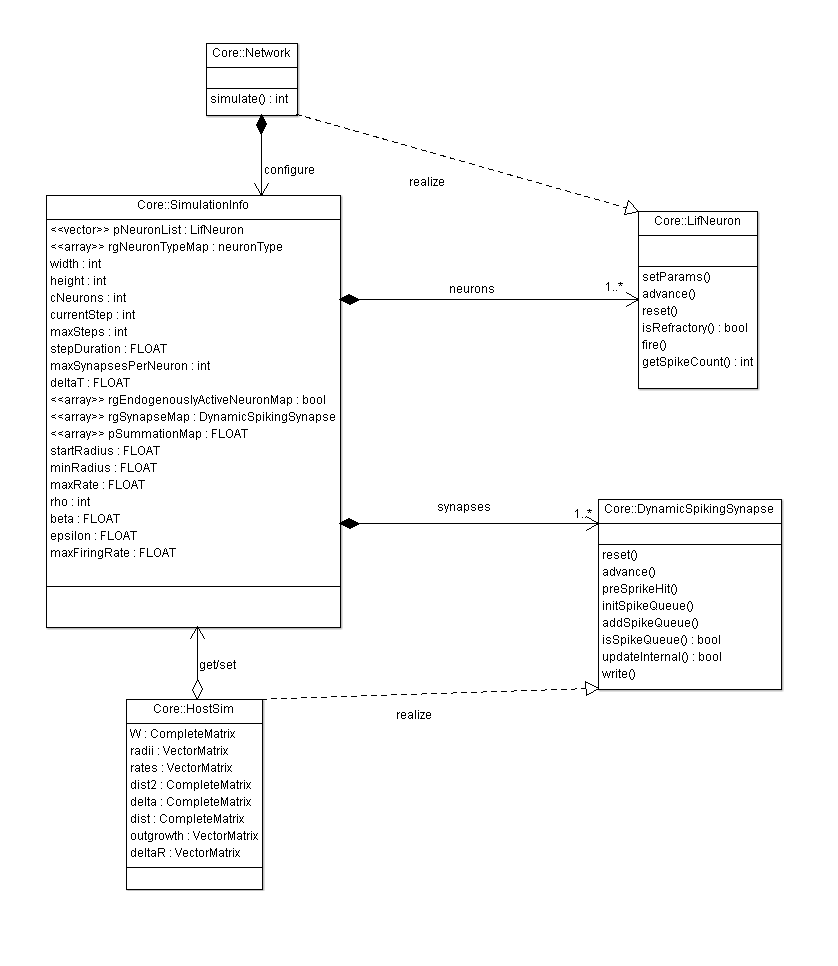
\includegraphics[width=.6\textwidth]{./diagrams/OldDiagram.png}
		\caption{BrainGrid's old design}
\end{figure}
\pagebreak

\noindent \mdseries The refactoring process of BrainGrid reorganized the data structures of the legacy code in order to implement a simpler program structure that prioritizes separating the model-dependent code from the model independent. The new code also stripped away some of the object-oriented structure of the neurons and the synapses, and instead now uses a data-centric structure, which utilizes two different structs as the containers of all neuron and synapse data. This structure was originally designed for the GPU implementation of the simulator, and this refactored version of the simulator simply uses that design for all other implementations as well. This is to simplify transitioning from single-threaded to multi-threaded.

\begin{figure}
	\centering
		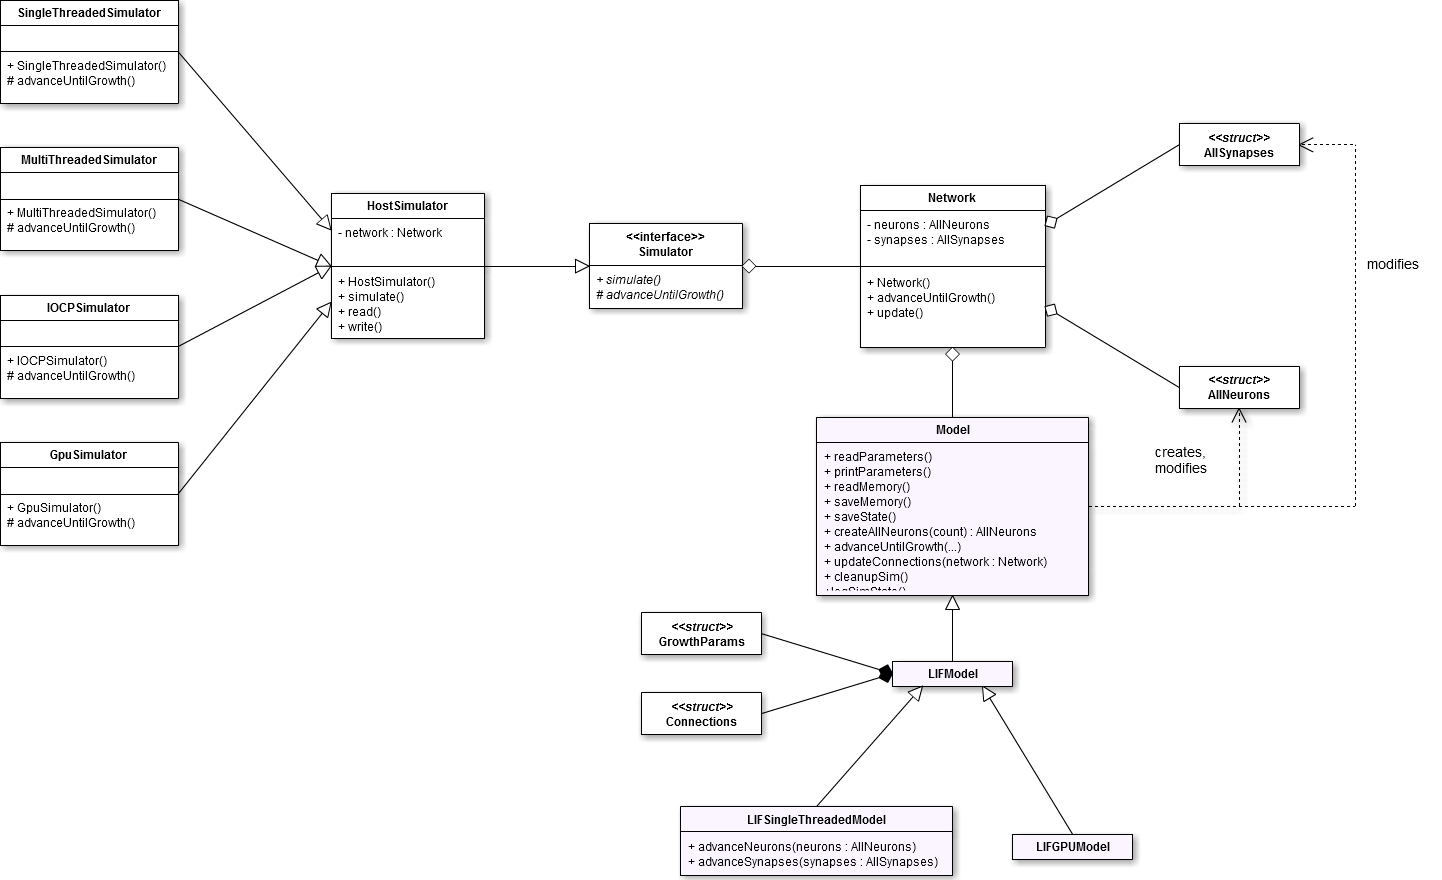
\includegraphics[width=\textwidth]{./diagrams/NewDiagram.png}
		\caption{BrainGrid's new design}
\end{figure}
\pagebreak


%------------------------------------- Features Section
\mdseries 
\section{Features}
\begin{itemize}
	\item Multiple simulation architectures:
	\begin{itemize}
		\item	Single-threaded
		\item Multi-threaded
		\item GPU (CUDA)
		\item GPU (AMP)
		\item GPU (OpenMP) --not yet implemented--
		\item GPU (IOCP) --not yet implemented--
		\item GPU (OpenCL) --not yet implemented--
	\end{itemize}
	\item Supported operating systems:
	\begin{itemize}
		\item Microsoft Windows
		\item Linux Distributions
	\end{itemize}
	\item Tools
	\begin{itemize}
		\item GitHub
		\item MATLAB
	\end{itemize}
\end{itemize}
\pagebreak


%------------------------------------- User Guide Section
\section{User Guide}
\subsection{Linux Distributions}
\mdseries Upon downloading and extracting the contents of the project, the following steps should be followed to run the simulation.
\begin{enumerate}
	\item	In a terminal window, navigate to the main project folder. 
	\item Run the \verb|make growth| command, which will compile the entire project.
	\item Upon completion, run the command \verb|./growth -t <input file>| where \verb|<input file>| is the full address of the configuration file, examples of which were in the \verb|config| folder.
	\item The program will then run and display the current step and epoc of the simulation. The output of the simulation (after the end of the simulation) will be saved in the \verb|output| folder. 
\end{enumerate}
\subsubsection{Advanced Use}
\mdseries Use of the UNIX command \verb|screen| is recommended in order to allow the process to run in the background. As the simulation is running, the \verb|Ctrl+A and D| keys will detach the currently running screen. The simulation will continue running in the background, while recording the output of the simulation to the seperate screen. At this point the user is free to log out of the machine.  To resume viewing the seperate screen, log back into the machine and use the command \verb|screen -r|.  This reattaches the screen.  As you might imagine using the unix \verb|screen| tool is essential to running the simulation on a remote machine. 

\noindent \mdseries For advanced users, the GCC compiler offers multiple optimization options that may provide some additional speed boost for the CPU-side simulation. It is recommended that, for each level of optimization, the output be verified against unoptimized/less optimized output. The BrainGrid team \bfseries DOES NOT \mdseries recommend using any optimization levels above -02. This level of optimization seems to be unstable, and does not seem to maintain consistent output results.   

\subsection{Microsoft Windows}
TODO
\pagebreak


%------------------------------------- Implementing Other Models Section
\section{Implementing Other Models}
TODO
\pagebreak


%------------------------------------- Tools Section
\section{Tools}
\subsection{GitHub}
\mdseries GitHub is a source-control system oriented towards the open source community. It offers multiple different features that are advantageous for the project, the most important of which the ability to manage multiple separate versions of the project’s code. This allows the project’s developers the ability to tackle multiple different features and/or bugs.

\noindent \mdseries In order to use GitHub, several tools have been released. The Microsoft Windows, Apple Macintosh software are available on their website.  On Linux distributions, the console is used to manipulate code. As such, the following are instructions on how to install and use GitHub on Linux distributions, focusing on the Ubuntu variety. These instructions assume that the user has already registered with GitHub.

\noindent \mdseries First, the operating system must be updated, and then use apt-get to install GitHub:

\begin{verbatim}
sudo apt-get update
sudo apt-get install git
\end{verbatim}

\noindent \mdseries Next, the username and email settings must be configured properly. 
\begin{verbatim}
git config --global user.name <USERNAME HERE>
git config --global user.email <EMAIL HERE>
\end{verbatim}

\noindent This is when the source code needs to be downloaded from the remote repository. Navigate to the folder where the source code is to be held:
\begin{verbatim}
git clone git://github.com/UWB-Biocomputing/BrainGrid.git
\end{verbatim}

\noindent \mdseries Once the source code is downloaded, the BrainGrid subfolder will be where all the code modifications will occur. Navigate to this subfolder, and use:
\begin{verbatim}
git branch -r
\end{verbatim}

\noindent \mdseries To view the multiple available remote branches (different variations of the code that exist outside the local computer). The GitHub webpage will contain more information about each branch, and how the source code varies in between them. In order to checkout a remote branch, use:
\begin{verbatim}
git branch <LOCAL NAME> origin/<REMOTE BRANCH NAME>
\end{verbatim}

\noindent \mdseries Where \verb|<LOCAL NAME>| is the name that will represent the local copy of the code. Once this is done, switching in between different local branches can be done by using:
\begin{verbatim}
git checkout <LOCAL NAME> 
\end{verbatim}

\noindent \mdseries To update a local branch with code on the remote version of the branch, use:
\begin{verbatim}
git pull
\end{verbatim}

\noindent \mdseries To save the modifications to the local branch, use:
\begin{verbatim}
git commit -a -m "`<MESSAGE HERE>"'
\end{verbatim}

\noindent \mdseries To move those changes to the remote branch, use:
\begin{verbatim}
git push
\end{verbatim}

\noindent \mdseries Note that Git will prompt the user for additional information.

\subsection{Matlab}
\mdseries For users with MathWork's MATLAB, a subfolder is included with the some sample files that correctly parse BrainGrid's output for use in MATLAB. The project currently only supports output generation during the end of the simulation, but pseudo real-time output may be implemented in the future.
\pagebreak


%------------------------------------- FAQ
\section{F.A.Q.}
\bfseries What version of CUDA does the project currently support?

\noindent \mdseries TODO

\noindent \bfseries 

\pagebreak


%------------------------------------- Acknowledgements
\section{Acknowledgements}
\mdseries The BrainGrid project has been designed, coded and refactored by multiple individuals over the years. The project has only moved forward thanks to these individuals, who have participated in this team as a labor of love. Those involved include, but are not limited to, the following list:
\begin{itemize}
	\item	Michael Stiber
	\item Fumitaka Kawasaki
	\item Paul Bunn
	\item Chris Burgess
	\item Derek McLean
	\item Hugo Ribeiro
\end{itemize}


\end{document}
